\documentclass{szzclass}

\topic{Konceptuální modelování, jeho význam, základní pojmy a způsoby modelování reálného světa.}
\code{BI-WSI-SI-05}
\subject{KOM}

\begin{document}

\tableofcontents
\newpage

\section{Konceptuální modelování}

Konceptuální modelování slouží k popisu reality a pochopení domény, kterou modelujeme.
Pomocí konceptuálního modelování může zjednodušit a navrhnout automatizaci určitých úkonů.
Z konceptuálního modelování lze poté přejít již k samotnému návrhu aplikace, například OntoUML je nástroj konceptálního modelování,
který lze jednoduše přeložit na UML (Unified Modeling Language). Díky tomu může analytik připravit v OntoUML model, který si
poté programátor převede do UML a na základě kterého napíše danou aplikaci.

\subsection{Pojmy}

\begin{itemize}
    \item Abstrakce
          Zjednodušení od nepodstatných detailů. Pracujeme s koncepty namísto skutečných věcí (konceptualizace).
          Koncepty reprezentuje dohodnutými symboli, které tvoří jazyk.
    \item Jazyk
          Jazyk může být textový, grafický nebo smíšený.
    \item Formální konceptualizace
          Oproti neformálním konceptuálním modelům, které jsou dnes běžně používané, mají formální modely
          výhody v přesnosti a možnosti je validovat a simulovat postup, který reprezentují, což zvyšuje jejich kvalitu.
          Tyto modely lze poté transformovat na návrhové modely (OntoUML -> UML) nebo rovnou přenést do implementace.
    \item Ulmannův trojúhelník
          Symbolizuje vztah mezi věcí, realitou a konceptualizací.
          \begin{figure}[ht]
            \centering
            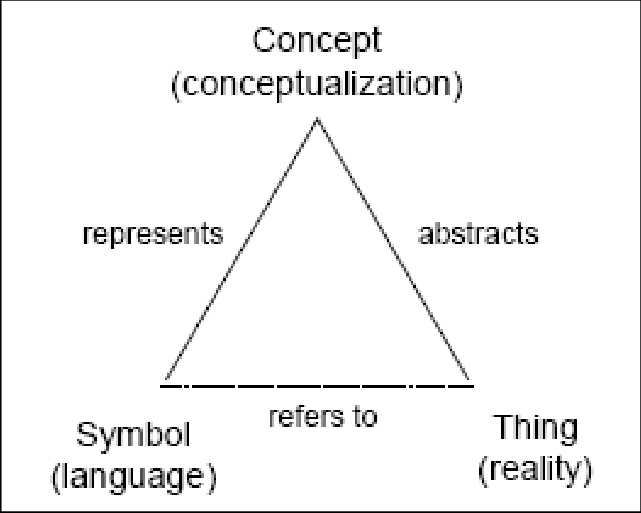
\includegraphics[width=0.5\textwidth]{topics/bi-wsi-si-05/ulmanns_triangle.png}
            \caption{Ulmannův trojúhelník}
          \end{figure}
\end{itemize}

\subsection{OntoUML}

OntoUML je jedním z možných nástrojů konceptuálního modelování pro popisování reálného světa. Narozdíl od UML nepopisuje třídy a objekty
z programátorského hlediska, místo toho definuje objekty podle jejich vlastností a stavů.
Součástí OntoUML je Unified Foundational Ontology (UFO), ta se dělá na tři části:
\begin{enumerate}
    \item UFO-A: strukturální aspekty reality - objekty, jejich typy, podčásti a role (v OntoUML se jedná o sortály)
    \item UFO-B: dynamické aspekty - události, jejich části a vazby mezi nimi (non-sortály)
    \item UFO-C: sociální aspekty - cíle, vztahy, stavy
\end{enumerate}

Používá modální logiku (rozšíření predikátové logiky):
\begin{itemize}
    \item existenční kvantifikátor
    \item univerzální kvantifikátor
    \item nutnost - ve všech světech platí
    \item možnost - v některém světě platí
\end{itemize}

\subsection{DEMO}

\end{document}
